\documentclass[11pt]{article}

\usepackage[margin=1.1in]{geometry}
\usepackage[T1]{fontenc}
\usepackage{mathpazo}
\usepackage{microtype}
\usepackage{amsmath,amssymb,amsthm}
\usepackage{booktabs}
\usepackage{graphicx}
\usepackage[section]{placeins}
\usepackage[font=small,labelfont=bf]{caption}
\graphicspath{{figs/}}
\usepackage{enumitem}
\usepackage[hidelinks]{hyperref}
\urlstyle{same}
\hypersetup{
  pdftitle={Making Thought Visible: Goodnow, Fan, and the Two Directions of a Drawing},
  pdfauthor={Flyxion},
  pdfsubject={Children's drawing, visual abstraction, and the process theory of inscription},
  pdfkeywords={children's drawing, Goodnow, Fan, visual abstraction, admissibility, sequence, cognitive tools}
}

\newtheorem{definition}{Definition}
\newtheorem{proposition}{Proposition}
\newtheorem{conjecture}{Conjecture}
\theoremstyle{remark}
\newtheorem*{remark}{Remark}
\newtheorem*{example}{Example}

\newcommand{\A}{\mathcal{A}}
\newcommand{\M}{\mathcal{M}}
\newcommand{\Sset}{\mathcal{S}}
\newcommand{\U}{\mathcal{U}}
\newcommand{\Pset}{\mathcal{P}}

\setlength{\parskip}{0.35em}

\title{\textbf{Making Thought Visible}\\[0.4em]
\large Goodnow, Fan, and the Two Directions of a Drawing}
\author{Flyxion\\ \small Independent Researcher}
\date{September 28, 2026}

\begin{document}
\maketitle

\begin{abstract}
\noindent
Jacqueline Goodnow and Judith Fan are separated by nearly fifty years, yet both treat children's drawings as organized cognitive achievements rather than defective pictures awaiting adult realism. Both also assign drawing a reciprocal epistemic function. For Fan, a drawing makes otherwise inaccessible structure (a category, a mechanism, a data relation) visible to a viewer. For Goodnow, the order and arrangement of a child's marks make otherwise inaccessible cognitive organization visible to the researcher. A drawing therefore faces in two directions: outward toward what it represents, and backward toward the activity that produced it. This essay argues that the two programs offer complementary decompositions of the same act. Goodnow decomposes a drawing into recurring graphic units and the order in which they are produced; Fan decomposes it into semantic parts and the distinctions they allow a viewer to recover. The difference is not between qualitative and quantitative research, nor between an obsolete and a modern psychology, but between a theory of how a drawing can be continued and a theory of what it can communicate. Three problems organize the comparison: decomposition (what counts as a unit), continuation (what may follow the marks already made), and address (which distinctions another mind must be able to recover). A formal treatment of continuation shows that, when marks accumulate without erasure, the images reachable by a drawer depend on order as well as on value, and that measures defined on finished images cannot establish that two drawers, human or artificial, share an abstraction policy. Children's drawings are organized twice: prospectively, by rules governing which marks can follow those already made, and retrospectively, by the distinctions a viewer can recover from the completed image. Neither organization alone yields a theory of graphic development.
\end{abstract}

\clearpage
\tableofcontents
\clearpage

\section{Two Directions of a Drawing}

A drawing is usually discussed as a picture of something. It stands for an object, a scene, a category, or a relation, and it succeeds or fails according to whether a viewer can recover what it stands for. That is the outward direction. There is also a backward direction, less often theorized, in which the drawing is a residue of the procedure that produced it. The order of the strokes, the places where a line stops short to avoid another, the region where something was squeezed in because the obvious space was already taken: these are traces of decisions that are not themselves depicted.

The two directions correspond closely to two research programs. In a colloquium titled ``Cognitive Tools for Making the Invisible Visible,'' Judith Fan describes a program built around the outward direction \cite{fancolloquium}. Human intellectual history, on this view, is bound up with the invention of external artifacts, such as number lines, Cartesian coordinates, diagrams, and data visualizations, that extend thought by making otherwise invisible structure perceptible. The research question is how people discover and communicate useful abstractions, and how they choose, from the enormous space of possible marks, those that will make some structure available to another mind \cite{fan2023versatile}. Jacqueline Goodnow's earlier work treats the backward direction as primary. Her question is what the arrangement and sequence of a child's marks reveal about the rules the child is using to build a figure and partition a surface \cite{goodnow1977,goodnow1973grammar}. She named the orientation in the title of a short paper, \emph{Visible Thinking} \cite{goodnow1978visible}.

The phrase ``making thought visible'' initially sounds like a description of Fan's program alone, since diagrams and explanatory sketches are instruments for exposing structures a viewer cannot otherwise see. But it describes Goodnow's method as well. The child's drawing is, for the researcher, an instrument for exposing a procedure that neither the child nor the researcher can inspect directly. A diagram can externalize an invisible mechanism; the order and arrangement of a child's marks can externalize an invisible procedure.

This reciprocity marks a point where two theories of the same activity need each other. A semantics of useful information explains why some marks are worth making. A process theory of inscription explains which marks are still available to be made. The comparison could be written as a story of succession, with Goodnow's classical descriptions updated by Fan's computation. That story is wrong in two ways. It misdescribes Goodnow, whose methods already included counted distributions, experimental interventions, and explicit tests of competing principles. And it misdescribes the relation between the programs, since Fan does not answer Goodnow's questions more precisely but asks a different question about the same act. A compact statement of the relation is this: Goodnow showed how drawing could be analyzed as having a syntax; Fan shows that this syntax is answerable to an audience. The developing child learns not merely how to make a form, but how to make a form carry a distinction.

The essay proceeds as follows. Section~\ref{sec:tradition} places both programs against the older traditions that judged children's drawing by resemblance, stage, or projective content. Sections~\ref{sec:goodnow} and~\ref{sec:fan} reconstruct each program from its primary sources. Section~\ref{sec:decomp} develops the claim that they offer different decompositions of a drawing. Section~\ref{sec:problems} organizes the comparison around the problems of decomposition, continuation, and address, and introduces a common selection model. Section~\ref{sec:continuation} formalizes continuation. Sections~\ref{sec:endpoint} through~\ref{sec:probes} draw consequences for evaluation, criticize each framework from the standpoint of the other, and propose measures that reach the process. Section~\ref{sec:tools} widens the argument from pictures to diagrams and plots.

A note on sources. Goodnow's \emph{Children's Drawing} is cited throughout from the 1977 Fontana/Open Books edition in The Developing Child series, edited by Jerome Bruner, Michael Cole, and Barbara Lloyd, whose pagination differs from the American edition \cite{goodnow1977}. Page references are to that edition only.

\section{Beyond Resemblance}
\label{sec:tradition}

For much of the twentieth century, children's drawings were read through three lenses, each of which treated the finished image as the object of analysis.

The first lens was resemblance. A drawing was measured against the visible appearance of its referent, and development was the progressive reduction of the distance between them. Luquet's influential sequence from ``intellectual realism,'' in which the child draws what it knows to be there, to ``visual realism,'' in which it draws what can be seen from one viewpoint, has this shape \cite{luquet1927}. The child's transparent houses and folded-out tables are errors of a principled kind, but errors nonetheless, measured against a standard the child has not yet reached.

The second lens was diagnostic. Goodenough's Draw-a-Man test scored the presence of body parts and details as an index of intellectual maturity \cite{goodenough1926}. The drawing was a symptom of a capacity located elsewhere, and its features were counted without regard to how they were produced.

The third lens was projective. Machover and others read the size, placement, and emphasis of figure parts as expressions of personality and emotional conflict \cite{machover1949}. Here too the finished image was treated as a static surface on which inner states had been deposited.

Goodnow's book answers the second and third lenses directly. Because the same child uses a whole range of techniques within a single day, week, or month, she endorses Rhoda Kellogg's warning about ``how dangerous it is to use children's drawings, particularly a single drawing, as a measure of intelligence'' \cite[p.~46]{goodnow1977}. And where a projective reading would find special emotional significance in oversized hands, she proposes that ``a simpler and likelier explanation'' is the difficulty of anticipating the problems each new line creates \cite[p.~48]{goodnow1977}.

The three lenses share an assumption. Each treats the drawing as a product whose meaning can be read off its completed form, and each locates the source of that meaning somewhere other than in the activity of drawing: in the visible world, in a general intelligence, or in affect. Goodnow's redirection of attention was aimed precisely at this assumption. Fan's program, arriving much later and from the direction of cognitive science and machine vision, rejects resemblance as the natural standard for a different reason: a drawing that resembles its referent closely may be a worse tool for the purpose at hand than one that resembles it less. The two programs thus converge on the rejection of realism as the measure of graphic competence, while disagreeing about what should replace it. Sections~\ref{sec:endpoint} and~\ref{sec:critique} return to the question and argue that no measure defined on the finished image alone, resemblance included, can serve as the replacement.

\section{Goodnow: Children's Drawing}
\label{sec:goodnow}

\subsection{Drawing as work with lines and shapes}

Goodnow's first chapter defines its subject broadly. The research covers ``the usual children's pictures of humans, together with their copying of simple shapes (geometric or letter-like shapes) and their construction of maps,'' all of which are called drawing because we use the word ``wherever the essence of the task is work with lines and shapes on a flat surface'' \cite[p.~9]{goodnow1977}. The grouping is deliberate and consequential. It refuses to treat the child's picture of a person as a fundamentally different object from the child's copy of a triangle, and so it directs attention away from what the drawing depicts and toward the constructional problem the drawer is solving. It also makes her project surprisingly close to Fan's general notion of external representations as cognitive tools. Neither researcher restricts drawing to art, self-expression, or resemblance.\footnote{The book appeared in the United States under the title \emph{Children Drawing}, which puts the emphasis on the activity rather than the product even more directly.}

The introduction states the book's orientation in a single contrast. Old drawings, Goodnow observes, provide ``a record of change and of times past made from the child's own point of view,'' and they lead children who look back on them to ask ``Did I ever do things like that?'' rather than ``Did I ever look like that?'' \cite[p.~7]{goodnow1977}. The photograph invites a question about appearance; the drawing invites a question about action. That is the backward direction of a drawing in its most ordinary form.

\subsection{Sequence as a choice among next steps}

Early in the book Goodnow gathers precedents for treating a graphic construction as a sequence. She reports the argument that ``graphic constructions should be viewed as a sequence of steps, each step calling for a choice between alternative next steps,'' an argument developed in work on how children copy horizontal, vertical, and diagonal lines on a checkerboard and why diagonals are especially hard \cite[p.~23]{goodnow1977}.\footnote{Goodnow's note 14. The description matches Olson's work on the child's acquisition of diagonality \cite{olson1970}; the attribution should be checked against the note.} She also cites Marshack's analyses of Palaeolithic marks, in which ``the analysis of meaning depends heavily on the analysis of sequence, as indicated by brush-work and other technical signs of order'' \cite[p.~23]{goodnow1977}; \cite{marshack1972}. Her own figure on the same page shows how one child's sequence for drawing a person changed over two weeks, each stroke numbered by its position in the order.

Two points follow directly. The formulation ``a choice between alternative next steps'' is already a statement of what Section~\ref{sec:continuation} will call admissibility: at every point in a drawing there is a set of possible continuations, and the drawer's rules select among them. And the two-week figure shows that the same child, drawing the same kind of figure, can reach it by different routes. The visible product does not reveal how the child divided the body into working units, or that the division changed. The sequence does. If the finished image underdetermines the procedure, then a theory that attends only to finished images will systematically miss a layer of organization, a point that returns in Section~\ref{sec:endpoint} as a formal claim about evaluation.

\subsection{Economy: one unit, many uses}

Chapter~2, ``Drawings as patterns,'' begins with the observation that children ``often make repeated use of the same graphic unit, especially for arms and legs'' \cite[p.~34]{goodnow1977}. Her figure collects cases in which one unit serves for both arms and legs, for eyes and nose, or for ears, hands, and feet. Drawing on Arnheim, she argues that this is not poverty of vocabulary. ``Economy represents an achievement of visual thought, the discovery that the same unit can be used for more than one purpose''; Arnheim's example is a drawing in which a heart shape, in varying sizes and proportions, serves as eyes, ears, mouth, brooch, and arms. Goodnow's conclusion is that ``what may appear at first sight to be a limited vocabulary of units may represent a conceptual strength, a discovery of similarity'' \cite[p.~35]{goodnow1977}; \cite{arnheim1954}.

The same pages set out Rhoda Kellogg's account, in which scribbles are explored in various placements, developed into simple ``diagrams'' such as circles and rectangles, joined into ``combines'' and ``aggregates,'' and then narrowed to a few preferred combinations that ``they adapt to represent objects and people'' \cite[p.~35]{goodnow1977}; \cite{kellogg1969}. For Kellogg, children respond continually to the presence of order in a shape, and the units they remember and repeat are those with good visual form or good balance. The mandala, a closed form usually ovoid with crossed lines, is her favourite example, and suns or radials are a similar kind of form \cite[p.~36]{goodnow1977}. The accompanying figure is titled ``Patterns incorporating favourite units (such as radials or mandalas) into human figures'': a radial becomes a head with spiky hair or a hand, and a mandala becomes a torso.

These observations carry a consequence that will matter throughout. An elementary mark has no fixed pictorial meaning in isolation. A unit can be selected first for its form, because it is balanced, repeatable, and already mastered, and only then assigned a semantic role. The order of explanation can run from form to reference rather than from reference to form.

\subsection{To each its own boundary, to each its own space}

The chapter then turns to the relations of units to one another. Goodnow summarizes the free drawings of young children in a phrase: they ``seem to operate with two general principles: to each its own boundary, and to each its own space'' \cite[p.~44]{goodnow1977}. Parts tend to be fenced off from each other, overlaps are rare, and children often seem to prefer a kind of no-man's land between parts.

Against these principles stands the embracing contour, a single line that combines head and body, or body and limbs, into one area \cite[pp.~44--45]{goodnow1977}. Goodnow gives three reasons for treating the shift from separate units to embracing lines as significant. It opens up new qualities, since a static figure can become more fluid and expressive of movement. It is an intellectual shift as well as an artistic one, because the child ``must mentally have constructed not simply a list of parts but a number of interacting relationships between parts.'' And it bears some relation to age, although chronological age turns out not to be the most promising link \cite[pp.~45--46]{goodnow1977}. In American samples, continuous and all-embracing lines are used most at about age seven; with simple shapes, ``threading'' a contour as if it were a continuous thread rises and then falls.

\subsection{A problem solved is a problem created}

The more profitable link, Goodnow argues, is between embracing lines and end-results, ``especially those end-results that appear to us to be `errors''' \cite[p.~47]{goodnow1977}. When an embracing line is used for a human, the line is harder to control and the figure may come out bizarrely out of proportion. The effects are most striking when a child operates with two principles at once, drawing an embracing line and also incorporating within it a carefully counted set of five fingers; the result may look more like a large bird than a person \cite[p.~48]{goodnow1977}. A second consequence, she writes, ``exemplifies the saying: `a problem solved is a problem created.''' Once embracing lines are used, the hand is often omitted or reduced to a mitten shape; children who add hands onto the initial core produce hands like bunches of bananas or boxer's gloves; children who try to carry the width required for several fingers along the whole arm produce arms massive like a paddle or a tree-trunk.

Her interpretation of these results is the crux of the chapter. It is tempting, she notes, to infer from bird-winged humans that the child is misperceiving, or from oversized hands that they carry special emotional significance. ``A simpler and likelier explanation, however, would seem to be the difficulty of anticipating the problems that each new use of line turns out to create'' \cite[p.~48]{goodnow1977}. The passage rejects both the perceptual and the projective readings described in Section~\ref{sec:tradition}, and replaces them with an explanation in terms of what earlier marks do to later ones. Section~\ref{sec:continuation} formalizes exactly this: a mark can foreclose continuations that the drawer will later need, and the difficulty lies in anticipating the foreclosure.

\subsection{Interventions on inherited figures}

Goodnow does not rest the boundary principles on description. ``If a way of describing drawings is to be fully checked,'' she writes, one should be able to set up an experimental situation in which the principle can be shown to matter, and ``the demonstration should not be post hoc'': it should be possible to say before the drawings are made that they will be of a particular type \cite[pp.~49--50]{goodnow1977}. The distinction she draws is between ``free'' drawings and ``constrained'' drawings, in which children are deliberately faced with a problem of boundaries by being asked to complete a figure that invites the crossing of lines \cite[p.~44]{goodnow1977}. Both of the studies that follow predict in advance that children will attempt a variety of solutions in preference to overlapping.

\paragraph{Arms and hair.} As Kellogg had pointed out, ``children seldom draw both arms and hair on a head'' \cite[p.~50]{goodnow1977}. In a circle-and-sticks figure, arms, hair, and ears all compete for the space around the single circle, and one solution is omission. Goodnow's own anecdote makes the point vivid. She interpreted lines drawn from a single circle as hair and was told ``No, arms''; a week later her confident reading of the same lines as arms was corrected, ``No, hair''; on later occasions hair and arms appeared alternately, each leaving the scene when the other appeared. To block omission, children were given a partly drawn figure (one circle and two vertical sticks) and asked to add both arms and hair; in further conditions they added hair to a figure whose arms were already in the way, or arms to a figure whose hair was already in the way \cite[p.~51]{goodnow1977}. Of sixty preschoolers asked to add both parts, one third placed the arms out from the ``legs,'' whereas the same classes a year earlier had drawn arms from legs in only one tenth of their spontaneous circle-and-stick figures. ``So we can apparently shift the location of one part by putting two parts into competition for the same space.'' Among the children who drew both parts from the circle, only three crossed the lines of arms and hair \cite[p.~52]{goodnow1977}. When arms were already present, children added hair at steep angles, let the parts touch without crossing, or, in a particularly telling solution, declared the problem impossible and offered to add a hat instead, because there was no room for hair \cite[pp.~53--54]{goodnow1977}. When hair was already present, most children changed the usual angle of the arms or moved them farther down the figure. The studies thus ``test the strength of commitment that children have to the boundary principles suggested by their free drawings'' and begin to explain aspects of free drawings ``that might otherwise seem mysterious or be attributed to some oddity in children's perception of the world'' \cite[p.~54]{goodnow1977}.

\paragraph{The wheels of a train.} Children often draw legs or wheels in what has been called ``aerial perspective,'' two above the body and two below. N.~H. Freeman had shown that a child who drew an animal this way would place all four legs below the body when a rider already occupied the space above \cite[pp.~54--55]{goodnow1977}. Goodnow and Roslyn Dawes reversed the manipulation, pre-empting the lower space: children aged three to seven were given a carriage with two large wheels and told that the child who drew it ``wanted to put in two more wheels, but didn't know how to do it'' \cite[p.~55]{goodnow1977}. The request posed several demands at once. The new wheels should match the old ones in size and shape, attach to the underside without extending beyond it, and touch the same ground; meeting all of these requires overlap. Because overlap is rare in spontaneous drawing, other solutions were predicted, and they appeared: wheels placed above the carriage; wheels changed in size or shape; extra wheels placed at the side; and the extension of the train itself by new carriages that created new underside. Overlapping wheels appeared only once in a group of close to a hundred children. ``To meet one goal we will often sacrifice another,'' she concludes, and in the most striking solutions ``the problem has been overcome by redefining the initial constraints, the initial terms or premises that created the bind. In effect, the problem has been redefined and the difficulty wiped out'' \cite[pp.~55--56]{goodnow1977}.

These are counterfactual completion tasks. The child inherits a partial inscription and must find a continuation that the child's own rules permit. Which constraint gives way (non-crossing, matching size, anatomical placement, the presence of a part) reveals its rank in the child's system. A drawing produced from nothing shows only the path the child happened to take. A drawing completed from an imposed starting state shows how the child's rules respond when the ordinary path is closed. The results also show that a child may produce a drawing that is less realistic but more procedurally coherent. Arms from the legs, a hat instead of hair, wheels above the carriage: each protects a boundary rule at the cost of anatomical or physical fidelity. The deviation is the solution, not the error.

\subsection{From patterns to sequences}

Goodnow closes the chapter by summarizing what the concepts of economy, number of parts, type of line, and ``arrangements to allow each part its own boundary and its own space'' have achieved: many features of children's drawings may be attributed ``to the way they solve problems encountered in the course of achieving certain kinds of patterns or problems created by their own achievements'' \cite[p.~57]{goodnow1977}. She then widens the notion of pattern to physical and conceptual organization (how people distribute themselves in a bus or restaurant, how ideas form clusters and compartments) before turning to sequence.

Chapter~3 distinguishes pairing (both legs drawn as a pair completed before moving on), left-to-right order within a pair, and top-to-bottom order \cite[p.~61]{goodnow1977}. The left-right analysis illustrates her use of distributions. From 273 Sydney preschoolers aged three to five who produced a recognizable human when asked to ``draw a person,'' she takes every drawing of two restricted types: 39 figures consisting of a single circle and two stick legs, and 40 consisting of a circle and four sticks. Across the 79 drawings, four arrangements of sticks occurred 39, 33, 3, and 4 times \cite[p.~61]{goodnow1977}. The same chapter uses a later mark to read an earlier one. The placement of a belly-button depended on the relative sizes of the circle and the leg sticks: when the circle was longer, the button was usually placed within it; when the sticks were longer, it was placed between them. Placement of the belly-button, her caption says, ``may reveal whether circle or sticks represents the trunk'' \cite[p.~72]{goodnow1977}.

With Levine she had already described such regularities in copying as a ``grammar of action'': tendencies to start at the top, to start at the left, to draw vertical lines from top to bottom and horizontal lines from left to right, to keep a line going rather than lift the pen, and to anchor new strokes to strokes already present \cite{goodnow1973grammar}. The analogy to syntax was intended seriously. The same triangle can be produced by many sequences, so the regularities are evidence about the producer rather than the product, much as grammatical rules constrain which strings are produced from a larger set of possible strings.

\subsection{Conventional equivalents and conservative revision}

The last substantive chapters, ``Developing conventional equivalents'' and ``From old to new equivalents,'' extend the analysis to graphic forms that come to stand for features of the world by conventional correspondence rather than by copying \cite[chs.~5--6, pp.~112--149]{goodnow1977}. Equivalents are learned, shared, and revised, and their revision tends to be conservative: children modify accessory elements while preserving an established core, rather than rebuilding a figure from the ground up. Karmiloff-Smith later found a related pattern when she asked children to draw a house or a person ``that does not exist'': younger children's modifications were confined largely to the end of a fixed drawing sequence or to changes in the size and shape of elements, whereas older children inserted, deleted, and reordered elements more freely \cite{karmiloff1990}. A procedure can be inspected by observing which departures from it are available to the drawer.

\subsection{What carries forward}

Four features of Goodnow's account carry forward into the comparison. Its organization is local and sequential: it governs the next mark given the marks already present. Its constraints can conflict, so that a completed figure records a resolution among competing demands, and ``to meet one goal we will often sacrifice another.'' Its constraints are not reducible to the goal of depiction. And it already contains, in the phrase ``the difficulty of anticipating the problems that each new use of line turns out to create,'' a theory of how early marks limit later ones.

It also contains more of Fan's program than a successor story would suggest. Discussing one five-year-old boy's drawings over two months, Goodnow notes that he drew relatively complex people when they stood alone or were the stars of the scene (``my sister,'' ``me at a birthday party''), and much simpler figures when the action and its setting were the major features (``we climbed a hill,'' ``we walked in the sand''). The same child uses a whole range of techniques within a single day, week, or month, which is why Kellogg warned against using a single drawing as a measure of intelligence; and ``we might well suspect that units and arrangements will vary with the artists' purpose'' \cite[pp.~46--47]{goodnow1977}. The goal-sensitivity that Fan measures systematically is already named here.

\section{Fan: Drawing as a Cognitive Tool}
\label{sec:fan}

\subsection{The program}

Fan begins from a compatible rejection of realism, but places much greater weight on communication. Drawings are physical representations used to learn, solve problems, explain, and convey concepts, and drawing is a versatile cognitive tool rather than merely an artistic product \cite{fan2023versatile}. The experimental questions follow: which information a drawing preserves, which it suppresses, how those selections vary with the representational goal, and whether another person can recover the intended concept. Early work established that producing and recognizing drawings draw on shared object representations, and that practice drawing objects can sharpen their representation for recognition \cite{fan2018common}.

\subsection{Contextual flexibility}

A drawing is a few marks standing for a very rich referent, and something must decide which properties survive the reduction. Fan's answer is that the survivors are selected according to what the drawing is for. In reference games, people produce detailed, faithful sketches when they must pick out one exemplar from similar exemplars, and sparser drawings when they need only signal the category \cite{fan2020pragmatic}. A drawing made for a partner who has seen earlier drawings of the same object can be sparser than a drawing made for a stranger, because shared history carries part of the meaning \cite{hawkins2023resemblance}. The same object has no single best drawing. It has a best drawing for a goal and an audience.

\subsection{Depiction and explanation}

The clearest statement of this position is the distinction between depiction and explanation. In work led by Holly Huey, participants drew novel mechanical objects either so that a viewer could pick out the object, or so that a viewer could understand how it worked \cite{huey2023explanations}. Depictions preserved features useful for identifying the object. Explanations suppressed many of those features and instead preserved causal parts, functional relations, and motion, often marked with arrows and other symbols, while de-emphasizing background detail. Viewers extracted mechanistic information more readily from explanations and identified the specific object more readily from depictions.

This result blocks a tempting reduction of Fan's theory to recognizability. It would be easy to read her developmental work as a story in which drawings become progressively more recognizable with age. Recognizability is only one objective among several. The broader theory is that competent drawers learn which abstraction is useful for a particular epistemic or communicative purpose.

\subsection{Development at scale}

The most direct point of comparison with Goodnow is a study of more than 37,000 drawings of visual concepts produced by children aged two through ten, collected at a museum drawing station \cite{long2024parallel}. Drawings became more recognizable across development, and the increase reflected growth in category-diagnostic information that could not be reduced to effort or visuomotor improvement. Even drawings that viewers could not identify retained information about broad properties such as animacy and real-world size. Children's ability to recognize one another's drawings improved in parallel with their production. After filtering, the dataset contained 37,770 drawings of 48 categories from 8,084 sessions at a museum kiosk, with a tracing task included so that visuomotor control could be measured separately from the content of the drawings (Figure~\ref{fig:long-array}).

\begin{figure}[!htbp]
\centering
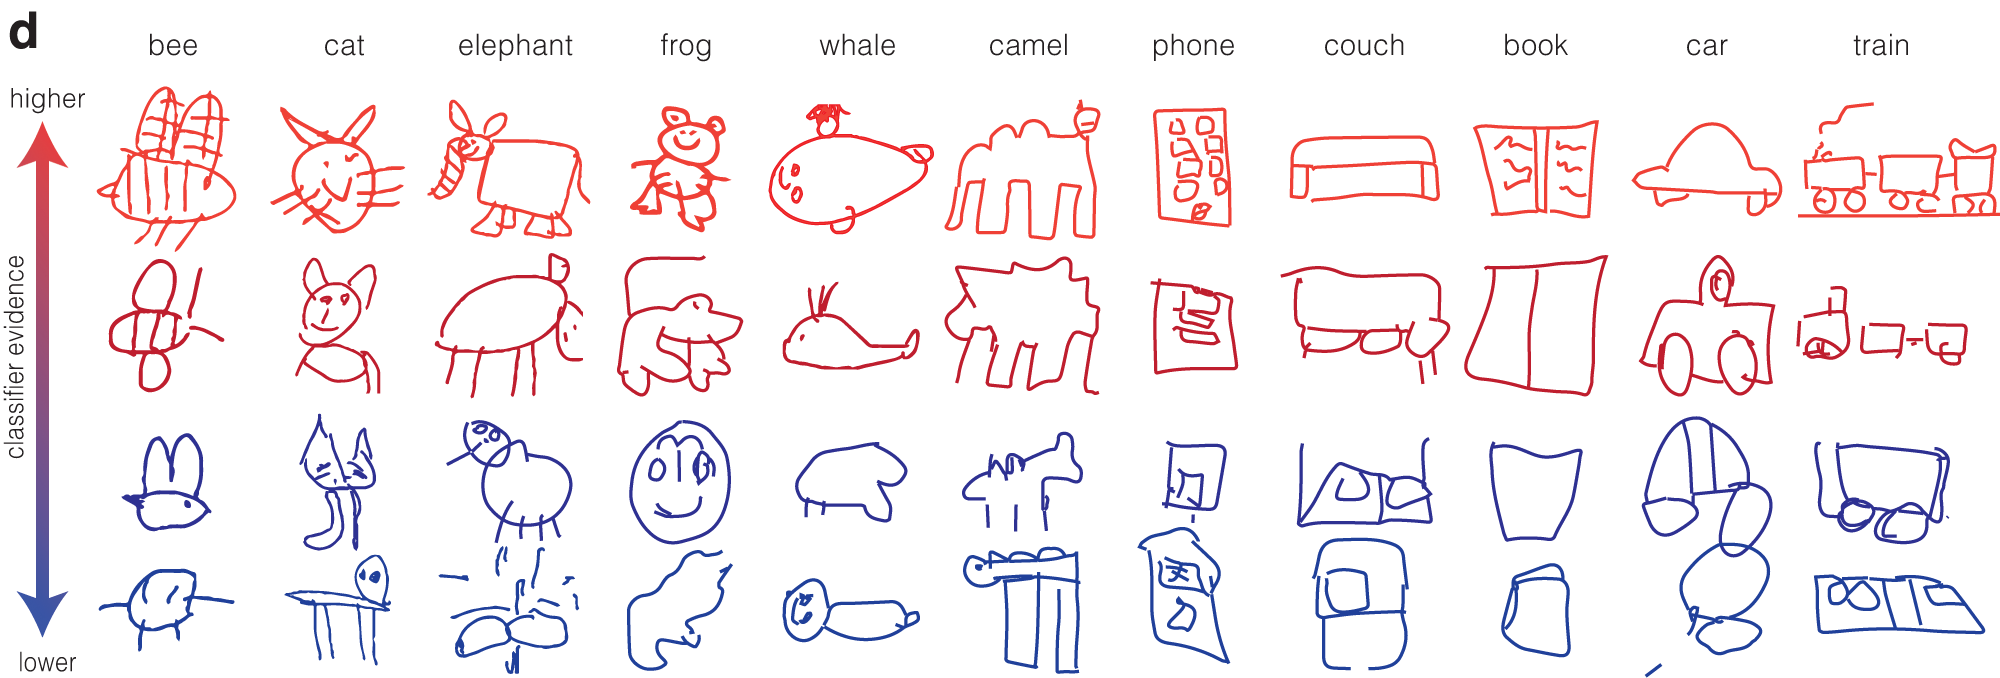
\includegraphics[width=\textwidth]{long_f1d.png}
\caption{Children's drawings from eleven of the 48 categories in the museum dataset, ordered from higher to lower classifier evidence for the intended category. Redder drawings carry more category-diagnostic information as measured by a vision model. Among the high-evidence trains is a figure of several carriages, each with its own wheels on a shared ground line. Source: Long et al.\ (2024), Fig.~1d, cropped; CC BY 4.0 \cite{long2024parallel}.}
\label{fig:long-array}
\end{figure}

The finding allows a reinterpretation of Goodnow's equivalents. A child's graphic equivalent is not merely a conventional mark substituted for a visible feature. It is a selective carrier of information whose adequacy depends on the distinctions a viewer must make. That a drawing unrecognizable at the level of category can still carry animacy and size shows that information is preserved at several grains at once.

\subsection{Machines and plots}

Two further strands of the program, both prominent in the colloquium, bear on the comparison \cite{fancolloquium}. The first concerns artificial systems. The SEVA benchmark collected human sketches of many object concepts under several production time limits, yielding for each concept a family of drawings ranging from detailed to very sparse, and compared how humans and vision models interpret them \cite{mukherjee2023seva}. It revealed a notable gap in how models and humans sparsify drawings under tight production budgets: a system can recognize sketches well while differing from humans in which content it treats as expendable \cite{mukherjee2023seva,vinker2022clipasso}.

The second strand concerns data visualization, which Fan treats as a cognitive tool for perceiving patterns too large, noisy, or slow to observe directly. Her group has compared humans and vision-language models on standard tests of visualization literacy. In the first study, the models underperformed all human cohorts and were highly sensitive to small changes in prompting \cite{verma2024}. In a larger follow-up with eight models, the models again performed worse than people on average, and although performance was correlated across test items, every model produced a pattern of errors reliably distinct from the human pattern \cite{verma2025}. A related study asked which graphs people judge effective for a given communicative goal. Participants favored graphs that contained the variables relevant to the question, but their choices were not reliably sensitive to more graded differences in how comprehensible the graphs actually were \cite{huey2023plots}. In the colloquium, Fan also described ongoing work on existing visualization literacy tests, aimed at assessments that diagnose specific misconceptions rather than yielding only a total score \cite{fancolloquium}.

Both strands turn on the same point. A total score, even a correlated one, can be produced by systems whose internal organization differs. That point is where Fan's program meets Goodnow's most directly.

\section{Three Decompositions of One Drawing}
\label{sec:decomp}

Goodnow's graphic unit and Fan's semantic part invite identification, since both name the pieces into which a drawing is divided. They are not the same kind of piece. Goodnow individuates units partly by their constructional recurrence: the oval that recurs as arm, petal, and foot is one unit. Fan's analyses tend to individuate parts by the object information they convey: the arm is a part because it carries information about the kind of thing depicted. A repeated oval may be one constructional unit while realizing several distinct semantic parts.

This suggests that a drawing has at least three non-equivalent descriptions.

\begin{enumerate}[leftmargin=2em]
\item Its \emph{graphic decomposition}: the units the drawer actually produces, grouped by constructional type.
\item Its \emph{semantic decomposition}: the parts or properties those units represent.
\item Its \emph{procedural decomposition}: the order in which the units are produced and the dependencies among them, such as which unit anchors which.
\end{enumerate}

\begin{definition}[Decompositions]
Let $\U$ be the set of graphic units in a drawing and $\tau : \U \to T$ assign each unit a constructional type. Let $\Pset$ be a set of semantic parts, and let a \emph{realization relation} $\rho \subseteq \U \times \Pset$ record which units realize which parts. Let $\prec$ be the production order on $\U$ and $\kappa \subseteq \U \times \U$ an anchoring relation, with $(u,v) \in \kappa$ when $v$ is attached to a boundary of $u$.
\end{definition}

The relations among the three descriptions are many-to-many, and Goodnow's pages supply an example of each. One graphic unit can realize several semantic parts: Arnheim's heart shape serves as eyes, ears, mouth, brooch, and arms \cite[p.~35]{goodnow1977}. Several units can jointly realize one part: a hand built from a palm and five counted strokes. One constructional type can realize parts of entirely different categories: a mandala, prized for its balance, becomes a torso, and a radial becomes a head of hair or a hand \cite[p.~36]{goodnow1977}. The same lines can even change semantic role while remaining graphically identical, as in the circle whose lines were ``No, arms'' one week and ``No, hair'' the next \cite[p.~50]{goodnow1977}. And two drawings with the same $\U$ and $\rho$ can differ in $\prec$ and $\kappa$, as in the child whose sequence for the same figure changed over two weeks \cite[p.~23]{goodnow1977}.

Fan's own annotation work shows the three descriptions pulling apart in practice. In the part-annotated subset of the museum dataset, annotators labeled each stroke with the object part it depicts (Figure~\ref{fig:long-parts}). Most strokes receive a single label. Some are marked as belonging to several parts at once, and some are marked as unintelligible. The first kind is a graphic unit realizing more than one semantic part; the second is a unit for which no realization could be agreed. Because the unit of annotation is the stroke, a pen-down-to-pen-up event, the scheme already records graphic units in something close to Goodnow's sense; what it does not yet analyze is the order in which those units were laid down and how each constrained the next.

\begin{figure}[!htbp]
\centering
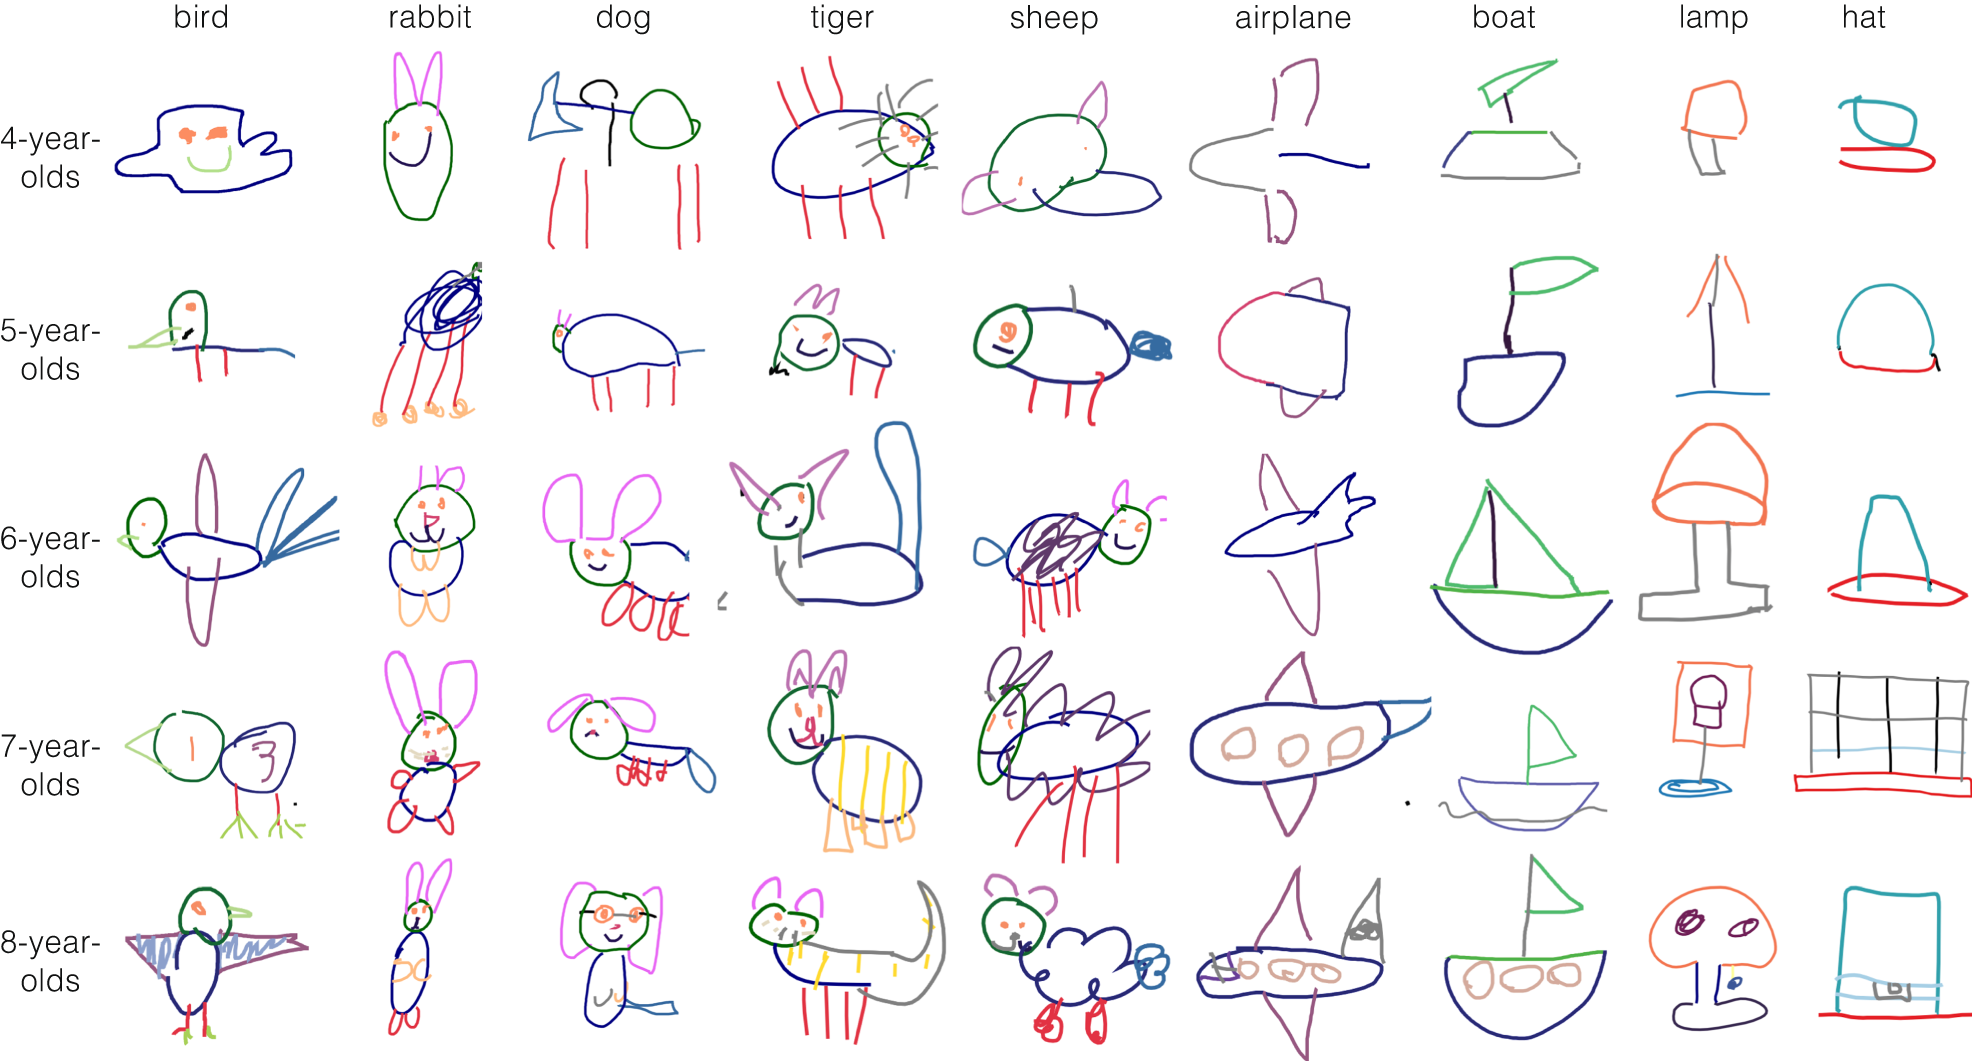
\includegraphics[width=\textwidth]{long_f4.png}
\caption{Part-annotated drawings by children aged four to eight. Each color is an object-part label agreed by human annotators; gray strokes were assigned to multiple parts, and black strokes were judged unintelligible. The gray strokes are single graphic units that realize more than one semantic part. The figure is reproduced to show stroke-level annotation; the key to individual part colors is given in the original article. Source: Long et al.\ (2024), Fig.~4; CC BY 4.0 \cite{long2024parallel}.}
\label{fig:long-parts}
\end{figure}

The decompositions can also be read off one another. Goodnow's belly-button analysis uses a later mark to recover the semantic role of earlier ones \cite[p.~72]{goodnow1977}. Among circle-and-stick figures, where a single circle carries the face and two sticks descend from it, it is not obvious from the image whether the circle is a head alone or a head and trunk combined, and so whether the sticks are legs or trunk and legs together. When children were asked to add a belly-button, the answer depended on proportions. Where the circle was long relative to the sticks, the button was usually placed inside the circle, below the face; where the sticks were long, it was usually placed between them, on the empty page. The first placement treats the circle as containing the trunk; the second treats the space between the sticks as the trunk, bounded by the sticks themselves. In the notation above, the placement of one unit discloses $\rho$ for the others. The researcher recovers the semantic decomposition not by asking what the drawing looks like, but by observing where the drawer's own rules put a diagnostic mark.

Goodnow is strongest on $\tau$, $\prec$, and $\kappa$. Fan is strongest on $\rho$ and on what a viewer can recover through it. The difference between them is therefore not between qualitative and quantitative research, nor between an obsolete and a modern developmental psychology. It is between two complementary decompositions of the same act: a constructional decomposition into marks and operations, and a semantic decomposition into parts and distinctions.

The decompositions also separate two axes of competence that endpoint measures tend to fuse. A child who reuses a small stock of constructional types across many semantic roles shows economy along $\tau$. A child whose drawings carry many diagnostic parts shows richness along $\rho$. These can vary independently. A measure defined over recognizability sees only the second, and will register the first only insofar as it happens to affect what a viewer can recover.

\section{Decomposition, Continuation, Address}
\label{sec:problems}

The comparison can now be organized around three problems rather than two biographies.

\paragraph{The decomposition problem.} What counts as a unit? Goodnow's units are discovered through repeated constructional forms and boundaries. Fan's parts are individuated by their semantic or category-diagnostic contribution. Section~\ref{sec:decomp} argued that both decompositions are real and that neither reduces to the other.

\paragraph{The continuation problem.} Given the marks already present, what additions remain possible without violating an established rule? This is Goodnow's particular strength, and her inherited-figure interventions are experiments on continuation.

\paragraph{The address problem.} Given an intended concept and a possible viewer, which distinctions must the drawing preserve? This is Fan's particular strength, and her manipulations of goal and audience are experiments on address.

The two programs can be placed in a single model. Characterize a drawing task by an existing graphic state $s$, a representational goal $g$, a possible audience $a$, and a repertoire of available operations $R$. Let $D(s \mid g)$ be the diagnostic value of a state (how well the marks on the page, taken together, convey the intended concept or mechanism) and $I(s \mid a)$ its interpretability for the anticipated viewer. Both are defined on states, and so on finished images, which are simply final states. The contribution of a candidate next mark $m \in R$ is then a marginal difference, $\Delta D(m \mid s, g) = D(s \oplus m \mid g) - D(s \mid g)$, and likewise for $\Delta I$, where $s \oplus m$ is the state after $m$ is added. A candidate mark has at least three kinds of value:
\begin{equation}
\label{eq:value}
V(m \mid s, g, a) \;=\; \alpha\, C(m \mid s) \;+\; \beta\, \Delta D(m \mid s, g) \;+\; \gamma\, \Delta I(m \mid s, a).
\end{equation}
Here $C$ measures constructional compatibility with the marks already present, $\Delta D$ measures the mark's contribution to diagnostic value, and $\Delta I$ its contribution to interpretability. The last term is the one most easily overlooked. In Hawkins and colleagues' studies, the same referent is drawn more sparsely for a partner who has seen earlier drawings of it than for a stranger \cite{hawkins2023resemblance}; a stroke that adds little for the first viewer may be indispensable for the second, although $D$ is unchanged. The terminal value of a finished drawing $x$ combines the last two terms,
\[
U(x \mid g, a) \;=\; \beta\, D(x \mid g) \;+\; \gamma\, I(x \mid a),
\]
while $C$ has no terminal counterpart: it constrains how an image is reached, not what it is worth once reached.

Goodnow's experiments chiefly expose $C$: whether a mark crosses a boundary, disrupts a pattern, occupies unavailable space, or violates a preferred sequence. Fan's experiments chiefly expose $D$ and $I$, and so $U$: whether a feature communicates category, exemplar, function, causal structure, or the distinction a particular audience needs. The division is not absolute. Fan's audience manipulations are manipulations of $I$, and her depiction versus explanation manipulation varies $g$ and hence $D$. Goodnow's inherited figures vary $s$ and hence $C$. Each program holds some terms roughly fixed in order to measure the others.

The coefficients cannot be treated as fixed developmental constants. They vary with the task. A child asked to copy a shape, draw a recognizable person, explain a mechanism, or complete a partially drawn figure is solving a different optimization problem in each case. Stage accounts read variation across a child's drawings as noise around a single level of competence. On a goal-sensitive view, apparent inconsistency may be adaptive variation in response to different goals. Goodnow already held this view. Her five-year-old who drew elaborate figures when they were the stars of a picture and simple ones when the action mattered more, and her suspicion that ``units and arrangements will vary with the artists' purpose,'' state the principle, and her inherited figures treat the child's output as a function of the problem posed \cite[pp.~46--47]{goodnow1977}. What Fan adds is the machinery to make the goal an experimental variable, to measure what changes with it, and to evaluate the result by what a viewer can recover.

Equation~\eqref{eq:value} also makes visible a conflict that neither program states on its own. The same alteration can have opposite values under the two criteria. Moving the arms down the body protects a boundary rule and raises $C$, while displacing a diagnostic relation and lowering $D$. An explanatory arrow that crosses the outline of an object raises $D$ for a mechanistic goal while violating exactly the non-crossing preference that Goodnow's children defended. A drawer is not maximizing one quantity. It is negotiating between what can be continued from the marks already made and what another person will be able to recover from the result.

As a theory of drawing, however, equation~\eqref{eq:value} is incomplete in a specific way. It scores a single mark against a fixed state. It says nothing about how the state came to be what it is, or how the present choice changes what will be possible next. That omission is where Goodnow's emphasis on sequence becomes indispensable.

\section{Continuation: Admissibility, Licensing, and Foreclosure}
\label{sec:continuation}

Replace the soft compatibility term $C$ with a harder notion. Let $\M$ be the space of possible marks and $\Sset$ the space of graphic states. A drawing is a sequence of marks $m_1, \dots, m_n$ producing states
\[
s_0, \qquad s_t = s_{t-1} \oplus m_t,
\]
where $s_0$ is the initial surface (blank, or an inherited figure) and $\oplus$ denotes adding a mark to the page. Marks accumulate. In the settings Goodnow studied, and in most fast sketching, they are not erased.

\begin{definition}[Admissibility]
An \emph{admissibility map} $\A : \Sset \to 2^{\M}$ assigns to each state the set of marks the drawer's constructional system permits from that state. A sequence is \emph{admissible} if $m_t \in \A(s_{t-1})$ for every $t$.
\end{definition}

The admissibility map is a compact description of a Goodnow-style constraint system. Non-crossing removes from $\A(s)$ any mark that would cross an existing boundary. The preference for each unit in its own space removes marks that would enter an occupied region. An attachment rule restricts where appendages may begin. The relation to $C$ in equation~\eqref{eq:value} is direct. A hard admissibility map is the limiting case in which $C(m \mid s) = -\infty$ for every $m \notin \A(s)$; a graded $C$ over the marks inside $\A(s)$ recovers the soft version, in which some admissible marks are merely preferred to others. The hard version suffices to show what the single-step model misses.

Adding a mark changes the admissible set in two directions.

\begin{definition}[Licensing and foreclosure]
For a state $s$ and a mark $m \in \A(s)$, the \emph{licensed set} and the \emph{foreclosed set} are
\[
L(s,m) = \A(s \oplus m) \setminus \A(s), \qquad
F(s,m) = \A(s) \setminus \big(\A(s \oplus m) \cup \{m\}\big).
\]
\end{definition}

Marks are treated here as tokens: particular acts at particular places, not types of stroke. The mark $m$ is excluded from $F(s,m)$ only because, once made, that token is no longer a candidate. Another token of the same type (a second wheel, a second arm) may well remain admissible, and is then not foreclosed. With this convention, $m' \in F(s,m)$ implies $m' \notin \A(s \oplus m)$, which is the property used below.

A mark licenses when it creates a boundary, attachment point, or region that later marks can use. Drawing a torso licenses arms at the shoulders. A mark forecloses when it occupies space, closes a contour, or introduces a boundary that later marks may not cross. Goodnow's interventions can be read directly in these terms. Pre-drawn hair forecloses attachment near the head. The first wheels of the inherited train foreclose the obvious positions of the rest. The observation that arms attach to the head when no body is present is a statement about licensing: the only boundary available to anchor an appendage is the head's contour.

Order dependence follows immediately.

\begin{proposition}[Order dependence]
\label{prop:order}
Let $m, m' \in \A(s)$. If $m' \in F(s,m)$ while $m \in \A(s \oplus m')$, then the sequence $(m', m)$ is admissible from $s$ and the sequence $(m, m')$ is not. The two sequences contain the same marks but only one of them can be executed.
\end{proposition}

\begin{proof}
$(m', m)$ is admissible because $m' \in \A(s)$ and $m \in \A(s \oplus m')$ by hypothesis. $(m, m')$ is not, because $m' \in F(s,m)$ implies $m' \notin \A(s \oplus m)$.
\end{proof}

The proposition is elementary, but it establishes the structural fact the rest of the argument needs: under accumulation without erasure, the set of finished images a drawer can reach depends on the order in which marks are attempted, not only on which marks the drawer values. Diagnostic value is scored over images; admissibility is enforced over paths.

The two can come apart. Informally, the question is: given what is already on the page, what is the best drawing still attainable? Fix a budget $B$ of further marks, in keeping with the production limits discussed in Section~\ref{sec:probes}, and define the \emph{reachable value} of a state as
\[
\Omega_B(s) \;=\; \max \big\{ U(x \mid g, a) : x \in X_B(s) \big\},
\]
where $X_B(s)$ is the set of final images of admissible completions of at most $B$ marks from $s$, and $\Omega_B(s) = -\infty$ if $X_B(s)$ is empty. At any fixed resolution the repertoire of marks is finite, so under a finite budget the set of completions is finite and the maximum is attained. $\Omega_B(s)$ is the best terminal value still attainable from $s$; it depends on $g$ and $a$, which are suppressed in the notation. A mark can have high immediate value $V$ and still lower $\Omega_B$.

\begin{example}[Greedy foreclosure]
Suppose the goal is to show a figure holding an object. From the blank state, two marks are admissible: a large head $h$, with high immediate diagnostic value since heads are strong cues for the category \emph{person}, and a torso $b$, with modest immediate value. Drawing $h$ first, placed centrally and large, forecloses a torso of adequate size beneath it. Arms can still be attached to the head's contour, but a held object then sits beside the head, where it is easily read as a hat, a speech bubble, or a separate object. Drawing $b$ first licenses arms at the shoulders and a hand position that reads unambiguously as holding. A greedy policy that selects the admissible mark with the highest immediate value at each step chooses $h$ first and reaches an image with lower $U$ than a policy that chooses $b$ first, although both value the same features. In the notation above, $V(h) > V(b)$ but $\Omega_B(s_0 \oplus h) < \Omega_B(s_0 \oplus b)$.
\end{example}

The example is schematic, but it is close to Goodnow's own account of embracing lines. An embracing contour is a mark of high immediate value: it unifies the figure and makes it expressive. It also forecloses the attachment of hands and fingers of reasonable size, so that later marks come out as mittens, bunches of bananas, or paddle-shaped arms, or are omitted altogether. Her phrase for this is ``a problem solved is a problem created,'' and her diagnosis is ``the difficulty of anticipating the problems that each new use of line turns out to create'' \cite[p.~48]{goodnow1977}. In the present terms, the young drawer evaluates marks by their immediate value $V$ and does not compute $\Omega_B$.

The train study adds a move the single-step model cannot describe at all. Children who extended the train with a new carriage did not choose among the wheel positions the inherited figure allowed. They drew a mark whose purpose was to change what was allowed.

\begin{definition}[Licensing move]
A mark $m \in \A(s)$ is a \emph{licensing move} for a goal $g$ and audience $a$ if its immediate contribution $\beta\,\Delta D + \gamma\,\Delta I$ is negligible but $\Omega_{B-1}(s \oplus m) > \Omega_{B}^{\neg m}(s)$, where $\Omega_{B}^{\neg m}(s)$ is the best terminal value attainable from $s$ by admissible completions of at most $B$ marks that do not include $m$. Typically this is because $L(s,m)$ contains marks that no admissible continuation from $s$ could otherwise reach.
\end{definition}

The extra carriage is a licensing move, and it is the mirror image of the greedy head. The head has high immediate value and lowers what remains reachable; the carriage has almost no immediate value, since a train is no more recognizable for having two carriages, and raises what remains reachable. It creates new underside on which the wheels can be attached without overlap. This is what Goodnow calls redefining ``the initial terms or premises that created the bind'' so that ``the difficulty [is] wiped out'' \cite[p.~56]{goodnow1977}. The hat offered instead of hair is a different solution of the same family: it substitutes a part whose admissible region is not yet occupied. Neither solution is visible as such in the finished image, which simply shows a longer train or a person in a hat.

The shape of the foreclosure problem recurs wherever space is limited and marks cannot be withdrawn. It suggests a reinterpretation of her sequencing regularities. Starting at the top and at the left, drawing enclosing contours before their contents, and anchoring new strokes to existing ones do not obviously serve depiction; none of them makes the finished figure more recognizable than another order would. But each tends to keep future options open. Top-left starts preserve the largest contiguous free region for later marks under a left-to-right, top-to-bottom layout. Contours before contents fix the boundaries that interior marks must respect before those marks are committed. Anchoring guarantees that each new mark creates attachment points for the next.

\begin{conjecture}[Sequencing rules as option preservation]
\label{conj:option}
Across the drawing tasks typical of a given culture and writing system, the sequencing regularities documented by Goodnow and Levine function as low-cost heuristics that, at each step $t$, select among admissible successors a mark $m$ that approximately maximizes $\Omega_{B-t-1}(s_t \oplus m)$, without requiring the drawer to evaluate completions explicitly.
\end{conjecture}

The conjecture is the most speculative claim in this essay, and it has an obvious rival. The same regularities could arise from motor fluency and from the habits of writing, without having been selected, by learning or by anything else, for what they do to later options. Starting at the top left may simply be what a hand trained on left-to-right script does first. Goodnow's own cross-cultural work shows that writing does shape copying: comparing children and adults in the United States and Israel, she and her colleagues found common developmental trends together with specific differences traceable to the patterns taught for forming English and Hebrew letters, and a generalization from letter patterns that was strongest while writing was first being mastered and declined afterward \cite{goodnow1973direction}. That finding is compatible with both explanations, which is why the two need to be separated.

They make different predictions. On the option-preservation account, the regularities should weaken or reverse where they no longer preserve options: on very large surfaces where space is not scarce, in erasable media where foreclosure can be undone, and for layouts that develop from the center outward. On the motor-and-literacy account, they should persist in all three conditions, since the hand and the writing habit are unchanged. The erasable-medium case is especially clean. Tablet drawing with an undo function makes every foreclosure reversible at low cost, so the option-preservation account predicts looser sequencing and more exploratory first marks there than on paper, while the motor account predicts no difference; this comparison does not appear to have been made directly, and it would be easy to run with data of the kind the museum kiosk studies already collect. Further predictions are specific to the option-preservation account. Children with the least regular sequencing should more often produce figures whose diagnostic parts are displaced or omitted because of earlier commitments, a claim about the \emph{kind} of error rather than its frequency. In line with Goodnow's diagnosis, such errors should cluster after marks with high immediate value and large foreclosed sets, such as embracing contours. Licensing moves, which require anticipating a foreclosure and acting against it, should become more frequent with age. And where writing direction and layout pull apart, for instance in a right-to-left script on a page whose free space lies to the left, sequencing should follow the free space rather than the script. Van Sommers's detailed studies of stroke order in adults, which found strong but task-sensitive regularities of the same general type, suggest that the regularities are not specific to children \cite{vansommers1984}.

With admissibility in place, the relation between the two programs can be stated more exactly than the additive model allowed. Fan's objectives, combined in $U$, define what a finished drawing is worth. Goodnow's constraints define $\A$, and hence which finished drawings are reachable from a given start by a given drawer. A drawer's abstraction policy is the joint product of both: a choice of which features to preserve, executed through a path that must remain admissible. The child must negotiate two constraints at once, and development is an expanding ability to choose sequences of marks that remain constructible for the drawer while becoming discriminable for the viewer.

\section{Endpoint Equivalence}
\label{sec:endpoint}

The same structure explains a methodological result that appears in both programs.

Let $\phi$ map a sequence of marks to the finished image it produces, discarding order and timing. The map is many-to-one. For any image $x$, the fiber $\phi^{-1}(x)$ contains every sequence that ends in $x$, and different drawers may occupy very different regions of the same fiber.

\begin{proposition}[Invisibility of process to endpoint measures]
\label{prop:fiber}
Let $E$ be any evaluation that depends on a drawing only through its finished image, so that $E = f \circ \phi$ for some $f$. If two drawers produce the same distribution over finished images for a task, then $E$ assigns them the same value, whatever their sequences, admissibility maps, or reasons for preserving the features they preserve.
\end{proposition}

The force of the proposition lies in how many common measures satisfy its hypothesis. Recognition accuracy, similarity to a reference drawing, classifier-based measures of diagnostic information, and human judgments of quality are all functions of the finished image. None can distinguish two procedures that converge on the same output.

Fan's comparisons of humans and machines reach this conclusion from the side of artificial systems. If a model recognizes completed sketches reasonably well but does not sparsify them as humans do under limited budgets, then successful recognition does not entail possession of a human-like abstraction policy. The model may recover the intended category without representing which marks a human would regard as expendable. The visualization studies make the same point for plots: performance can be correlated with human performance across test items while the pattern of errors remains reliably unlike the human pattern \cite{verma2025}.

The same separation between aggregate success and human-like organization appears beyond drawing, in work Fan co-led on physical prediction. In the Physion benchmark, vision models that learn object-centric representations generally outperformed those that do not, yet still fell far short of human performance, while graph neural networks given direct access to the physical state of a scene both performed substantially better and made predictions more similar to those of human observers \cite{bear2021physion}. The authors conclude that extracting physical representations of scenes is the main bottleneck to human-like physical understanding in vision algorithms. The lesson carries over. Whether a system's answers resemble human answers depends on whether it represents the structure the task is actually about, not only on how many answers it gets right; comparable outputs need not arise from comparable representations or inferential procedures.

Goodnow supplies the developmental analogue. Two children may produce similar completed figures through different sequences and under different operative constraints, and one child may change sequence within two weeks while producing much the same figure \cite[p.~23]{goodnow1977}. One may reach a conventional person figure through a stable, anchored procedure; another may reach it through a sequence that happens to avoid foreclosure on this occasion and would fail under a small change of starting state. Behavioral equivalence at the endpoint does not establish procedural equivalence, and the inherited-figure method exists precisely because the endpoint alone cannot separate these cases.

Taken together, the two programs support a general claim about evaluation. Aggregate success can conceal differences in organization. A finished image is insufficient evidence about the system that generated it. To understand abstraction, one must study not only whether the output communicates, but what was removed, what was preserved, in what order, and under which constraints.

\section{What Each Framework Misses}
\label{sec:critique}

A productive comparison should also criticize each program from the standpoint of the other.

Goodnow's rule descriptions identify striking regularities without always providing a strong account of why one rule is preferable for a particular representational purpose. The grammar of action says that children tend to start at the top; it does not say what starting at the top is \emph{for}. Her discussion of boundaries, compartments, and order gestures toward functional explanation, but the functional criterion remains largely implicit. Fan's measures of recognizability and diagnostic information supply exactly such a criterion. They allow one to ask whether a rule helps or hinders the recovery of the intended distinction, and Conjecture~\ref{conj:option} is an attempt to state what a functional account of Goodnow's rules might look like when it is framed in terms of the options a rule preserves for later diagnostic marks.

Fan's endpoint measures, in turn, risk losing precisely what Goodnow preserved: the drawing as an irreversible temporal performance in which early marks constrain later possibilities. A theory trained only on completed images treats histories that end in the same image as equivalent, even when they disclose very different cognitive organizations. There is a second, subtler loss. The mandalas and radials that Goodnow discusses through Kellogg are chosen and repeated for their balance, unity, and contrast, not for what they refer to \cite[pp.~35--36]{goodnow1977}. When they are incorporated into human figures, a torso is drawn as a mandala and a hand as a radial because those are the forms the child has mastered and values. A category-diagnostic measure credits the resulting figure only insofar as the torso and hand are recoverable as torso and hand. It has no term for the fact that the form was selected first and the reference assigned afterward. The asymmetry is easy to state. A free-standing mandala has diagnostic value near zero for any object category. The same mandala placed beneath a head, with legs below it, contributes substantially to the figure's being read as a person. The diagnostic value changes completely between the two cases; the constructional achievement, a balanced closed form with crossed lines, does not change at all. Recognizability measures successful reference; it does not measure every kind of order a child has learned to produce. Making recognition the privileged dependent measure therefore tends to treat non-referential organization as noise, and to misdescribe drawings in which reference is borrowed by an already organized form.

The two criticisms are symmetric. Goodnow describes organization without a sufficient theory of its purpose; Fan measures purpose-relative success without a sufficient theory of the organization that produces it. Neither criticism is fatal, because each program supplies what the other lacks.

It is equally important to reject a false historical asymmetry. Goodnow is not the qualitative predecessor of a quantitative science. She used counted distributions (79 drawings sorted from 273, with type frequencies reported), comparisons across conditions and against baseline rates from the same classes a year earlier, partial-figure interventions, and predictions stated in advance, with the explicit requirement that the demonstration ``should not be post hoc'' \cite[pp.~50, 52, 61]{goodnow1977}. Fan did not invent the population-level study of recurring graphic structures. Her innovations lie in scale, in computational characterization of drawings, in recognizer-based evaluation, and in an explicit theory of communication. The continuity between the two is methodological seriousness. The difference is the level at which graphic organization is modeled.

\section{Measures That Reach the Process}
\label{sec:probes}

If endpoint measures cannot see the process, then measures that can see it have to be built from something other than single finished images. The two programs already contain the needed designs. Combining them yields a small family of probes that apply equally to children, adults, and machines.

\paragraph{Budget ladders.} Fan's use of production limits turns one drawing into a family. Let $x_b$ be the drawing produced under budget $b$ (time, strokes, or ink). The sequence of drawings under decreasing budgets reveals a priority ordering over features: what survives at every level is what the drawer treats as least expendable for the goal. Two drawers with identical full-budget drawings can have very different ladders, and comparing human and model ladders is more informative than comparing recognition scores at any single level.

\paragraph{Inherited-figure probes.} Goodnow's completion method turns one drawer into a response function. Present a partial figure $s_0$ chosen so that the drawer's usual path is blocked, and record the completion. Varying $s_0$ systematically maps $\A$: which constraints are honored, which are sacrificed, and in what priority. For sketch-generating models, the analogous test supplies a partial sketch that forecloses the model's typical composition and asks whether completions respect boundaries, relocate diagnostic parts, or simply overwrite what is already present. A system that overwrites has no admissibility structure in Goodnow's sense, whatever its accuracy on unconstrained generation. A system that never extends the train, never offers the hat, and never moves the arms to the legs has an admissibility structure but no licensing moves, and that too is a finding about its organization that no recognition score records.

A recent study shows that this design transfers readily to current methods. Philippsen, Tsuji, and Nagai gave children at a museum a tablet on which part of a drawing was already present, and let them draw freely \cite{philippsen2022}. Four categories were used (face, human figure, house, car), each in three configurations: an outline with no inner features, the inner features without an outline, and the inner features scrambled out of their usual arrangement (Figure~\ref{fig:phil-stimuli}). Adult raters scored each response for scribbling, coloring, tracing, and completion, and a convolutional network was used to characterize the drawings at local and global levels. Scribbling decreased and completion increased with age (Figure~\ref{fig:phil-responses}).

\begin{figure}[!htbp]
\centering
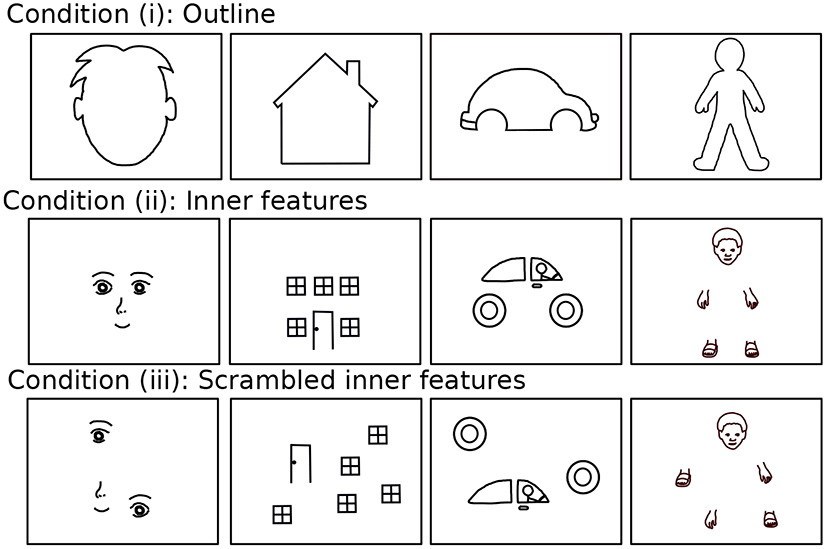
\includegraphics[width=0.78\textwidth]{phil_g1.png}
\caption{Inherited states in a drawing-completion task. Each child began from an outline, from inner features alone, or from inner features scrambled out of their usual configuration. Source: Philippsen, Tsuji, and Nagai (2022), Fig.~1; CC BY \cite{philippsen2022}.}
\label{fig:phil-stimuli}
\end{figure}

\begin{figure}[!htbp]
\centering
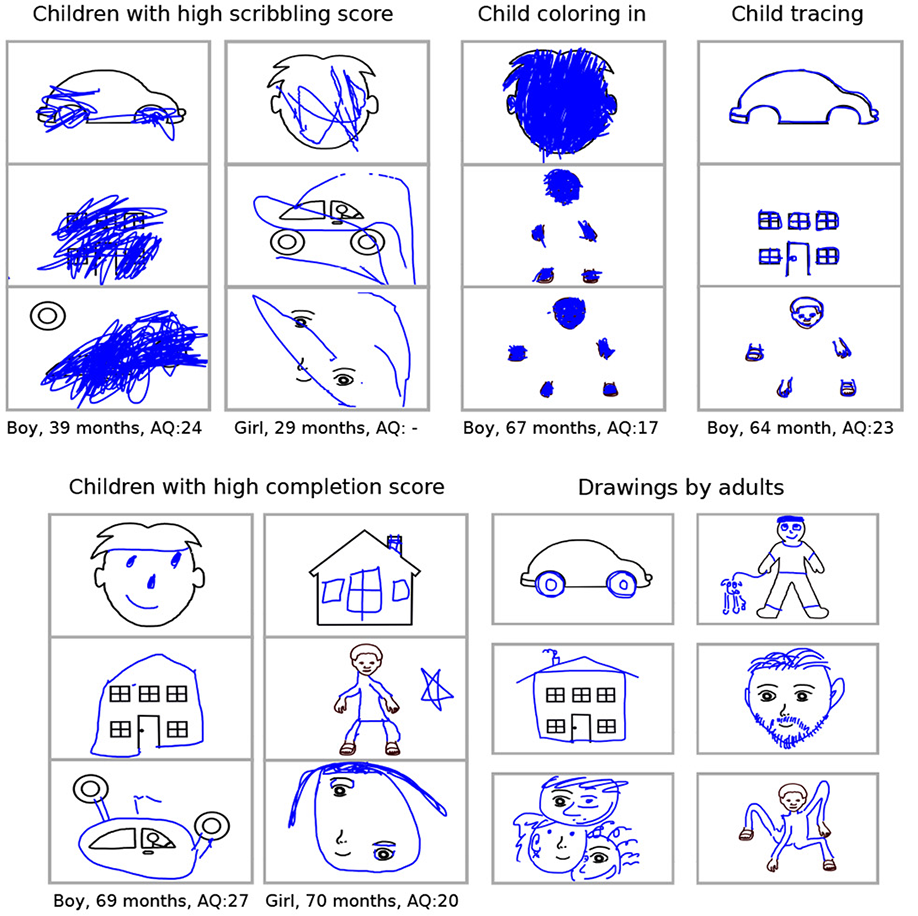
\includegraphics[width=0.86\textwidth]{phil_g4_stacked.png}
\caption{Responses rated high on scribbling, coloring, tracing, and completion, with adult drawings for comparison. The original single-row figure has been split into two rows for legibility. Each category names a relation between the child's new marks and the marks already present. Source: Philippsen, Tsuji, and Nagai (2022), Fig.~4; CC BY \cite{philippsen2022}.}
\label{fig:phil-responses}
\end{figure}

The three configurations map directly onto the continuation problem. An outline supplies the enclosing boundary first, the order Goodnow's children favored, and licenses interior features. Inner features alone reverse that order: the child must recognize the parts and supply a contour that fits them, which is the embracing-line problem posed from the other side. The scrambled condition breaks the arrangement the child's rules expect, and so functions like Goodnow's constrained drawings: the child must either reorganize the parts into an admissible figure or leave them unintegrated. The rating categories are also worth noticing. Scribbling over the inherited marks, coloring them in, tracing them, and completing them are not styles of image. They are relations between new marks and old ones, read off the finished drawing. The design is Goodnow's, the measurement is of the kind Fan's program developed, and the question it answers is how children continue a state they did not create.

\paragraph{Order logging.} Where the medium permits, record the sequence rather than only the result. Stroke order, pauses, and the timing of diagnostic parts relative to structural parts allow direct tests of Conjecture~\ref{conj:option}, and they allow drawers to be clustered by procedure rather than by output.

\paragraph{Game-based deployment.} The probes above are well suited to deployment as games. Allen and colleagues argue that games occupy a productive middle ground in the study of mind: they preserve substantial experimental control while eliciting extended, intrinsically motivated behavior in richer state spaces than conventional one-shot laboratory tasks \cite{allen2024games}. Fan's own work already uses the form, in communicative reference games and in the guessing game at the museum kiosk (Figure~\ref{fig:long-array}). A drawing game built on the present framework would present inherited partial figures, record every stroke, and vary obstruction, budget, audience, and communicative goal across repeated trials. It would then estimate a participant's admissibility map from a sequence of decisions rather than from a single finished image. The affinity runs deeper than convenience. A game and a Goodnow partial figure do the same thing: each builds a structured situation in which priorities that are normally invisible become observable. What a child does with the train shows not only whether the child can draw wheels, but which transformations of the page the child treats as permissible, useful, or disruptive under the conditions set.

\paragraph{Goal switching on a fixed referent.} Fan's depiction versus explanation design holds the referent fixed and varies $g$. Crossing it with inherited figures and budget ladders separates three sources of variation that endpoint studies confound: what the drawer is trying to convey, what the drawer can afford to draw, and what the page still allows.

\paragraph{Non-referential order.} Tasks with no referent at all, such as symmetric patterns, radials, and ornamental borders, measure organization along the constructional axis directly, without routing it through recognition. They give Goodnow's radials a place in an evaluation battery instead of leaving them outside it.

None of these probes requires a new theory of what drawings mean. Each requires only that the object of study be the mapping from task to drawing, rather than the drawing alone. Because each yields a profile for a single drawer (a ladder, a response function over inherited states, a sequence record), the probes also lend themselves to the study of individual differences and not only group-level development. Both programs already point this way: Goodnow tracked single children over weeks and months, and Philippsen and colleagues designed their completion task partly to quantify differences between individual children \cite{philippsen2022}.

\section{Diagrams, Plots, and the Two Directions}
\label{sec:tools}

Goodnow's decision to treat pictures, copied shapes, and maps as one activity and Fan's extension of drawing research to diagrams, graphs, and data visualizations point in the same direction. A cognitive tool is not merely an external store of thought that already exists in finished form elsewhere. Its spatial conventions determine which relations become perceptually available and which inferences become easy.

This is an established theme in the study of diagrams. Larkin and Simon argued that a diagram can be computationally superior to an informationally equivalent list of sentences because it indexes information by location, so that related facts sit near one another and can be retrieved by looking rather than searching \cite{larkin1987}. Tversky has traced how conventions of spatial layout, such as up for more, left to right for time, containment for membership, and lines for connection, recruit spatial reasoning for abstract content \cite{tversky2011}. A number line makes magnitude comparison a matter of relative position. A coordinate system makes covariation a matter of slope. A scatter plot makes the absence of a relation visible as the absence of shape.

The present framework adds a sequential point to this familiar one. Diagrams are also built mark by mark, and their conventions also license and foreclose. Choosing the axes of a plot forecloses some comparisons before any data are drawn. Placing a component at the center of a schematic licenses connections radiating from it and makes a linear causal chain harder to lay out. The designer of a visualization faces Goodnow's problem as well as Fan's: the design must preserve the relations the audience needs, and it must be constructible in an order that does not close off the space those relations require. Work from Fan's group on graph choice suggests that ordinary viewers are sensitive to the address problem in a coarse form, favoring plots that contain the variables a question requires, but less sensitive to finer differences in how well a plot supports comprehension \cite{huey2023plots}. The continuation problem suggests a complementary question: whether expertise in making diagrams consists partly in sequencing habits that preserve options for the relations one is likely to need.

The two directions of a drawing reappear here in a sharper form. In Peirce's terms, a diagram is an icon of relations: it represents by sharing relational structure with what it represents \cite{peirce}. The outward direction is not only iconic, however. Fan's work shows that it also rests on convention and on pragmatic inference: a sparse sketch can succeed for a partner because of a shared history that no resemblance explains \cite{hawkins2023resemblance,fan2020pragmatic}. The backward direction is indexical in a causal sense: the diagram is a physical residue connected to the choices that produced it. The outward direction, with its iconic, conventional, and pragmatic relations, is chiefly Fan's subject. The backward, indexical direction is chiefly Goodnow's. Every mark on a page carries both, and a theory that reads only one of them will attribute to the referent structure that belongs to the procedure, or to the procedure structure that belongs to the referent.

\section{Conclusion}

Jacqueline Goodnow and Judith Fan treat drawing as a technology for converting latent organization into visible form. Goodnow studies how graphic sequences disclose the child's rules for constructing and partitioning space. Fan studies how selective abstraction makes categories, mechanisms, and data relations available to another mind. Their work converges on a view of drawing as goal-sensitive compression, but differs over where its organization is chiefly sought: Goodnow locates it mainly in the admissible succession of marks, while Fan locates it mainly in the informational usefulness of the resulting representation. Each attends to the other's concern as well (Goodnow to purpose, Fan to production budgets), but the emphasis differs.

Children's drawings are therefore organized twice. They are organized prospectively, by rules governing which marks can follow those already made, and retrospectively, by the distinctions a viewer can recover from the completed image. Goodnow explains the first organization; Fan measures the second. A complete theory must join them, because what a drawing can communicate depends partly on what its prior marks still permit the drawer to do.

The formal contribution of this essay is to make that dependence explicit. An admissibility map encodes Goodnow's constraints; marks license and foreclose later marks; the images reachable by a drawer depend on order as well as on value; and ordinary sequencing regularities can be read as heuristics that preserve the options a goal will later require. The methodological contribution follows from the same structure. Because the map from procedures to finished images is many-to-one, measures defined on finished images cannot establish that two drawers, human or artificial, share an abstraction policy. Budget ladders, inherited-figure probes, order records, goal switching on fixed referents, and non-referential tasks can.

Fan does not supersede Goodnow, because an endpoint-oriented analysis of category information cannot by itself explain the constructive history that generated the endpoint. Goodnow does not anticipate Fan, because a description of constructional rules cannot by itself say which rules serve which purposes for which viewers. Each makes thought visible in one of the two directions a drawing faces: to a viewer, as a representation of something the drawer understands, and to a researcher, as a record of how that understanding was put onto the page.

This essay does not attempt the synthesis it calls for. It shows that the two programs are complementary, supplies a vocabulary in which their contributions can be stated together, and proposes measurements that would test the vocabulary. A theory of graphic development that actually joins them, specifying how admissibility maps change with age and how children come to anticipate foreclosure, remains to be built.

\begin{thebibliography}{99}
\small

\bibitem{allen2024games}
Allen, K., Br\"andle, F., Botvinick, M., Fan, J.~E., Gershman, S.~J., Gopnik, A., Griffiths, T.~L., Hartshorne, J.~K., Hauser, T.~U., Ho, M.~K., de~Leeuw, J.~R., Ma, W.~J., Murayama, K., Nelson, J.~D., van~Opheusden, B., Pouncy, T., Rafner, J., Rahwan, I., Rutledge, R.~B., \ldots\ Schulz, E. (2024).
Using games to understand the mind.
\emph{Nature Human Behaviour}, 8(6), 1035--1043.
\url{https://doi.org/10.1038/s41562-024-01878-9}

\bibitem{arnheim1954}
Arnheim, R. (1954).
\emph{Art and Visual Perception: A Psychology of the Creative Eye}.
Berkeley: University of California Press.

\bibitem{bear2021physion}
Bear, D.~M., Wang, E., Mrowca, D., Binder, F.~J., Tung, H.-Y.~F., Pramod, R.~T., Holdaway, C., Tao, S., Smith, K., Sun, F.-Y., Fei-Fei, L., Kanwisher, N., Tenenbaum, J.~B., Yamins, D.~L.~K., \& Fan, J.~E. (2021).
Physion: Evaluating physical prediction from vision in humans and machines.
\emph{Proceedings of the Neural Information Processing Systems Track on Datasets and Benchmarks}, 1.
\url{https://arxiv.org/abs/2106.08261}

\bibitem{fancolloquium}
Fan, J.~E. (2025, March 20).
\emph{Cognitive tools for making the invisible visible}.
Colloquium on the Brain and Cognition, Department of Brain and Cognitive Sciences and Center for Brains, Minds, and Machines, MIT Siegel Family Quest for Intelligence, Massachusetts Institute of Technology.
\url{https://www.youtube.com/watch?v=AF3XJT9YKpM}

\bibitem{fan2018common}
Fan, J.~E., Yamins, D.~L.~K., \& Turk-Browne, N.~B. (2018).
Common object representations for visual production and recognition.
\emph{Cognitive Science}, 42(8), 2670--2698.
\url{https://doi.org/10.1111/cogs.12676}

\bibitem{fan2020pragmatic}
Fan, J.~E., Hawkins, R.~D., Wu, M., \& Goodman, N.~D. (2020).
Pragmatic inference and visual abstraction enable contextual flexibility during visual communication.
\emph{Computational Brain \& Behavior}, 3, 86--101.
\url{https://doi.org/10.1007/s42113-019-00058-7}

\bibitem{fan2023versatile}
Fan, J.~E., Bainbridge, W.~A., Chamberlain, R., \& Wammes, J.~D. (2023).
Drawing as a versatile cognitive tool.
\emph{Nature Reviews Psychology}, 2, 556--568.
\url{https://doi.org/10.1038/s44159-023-00212-w}

\bibitem{goodenough1926}
Goodenough, F.~L. (1926).
\emph{Measurement of Intelligence by Drawings}.
Yonkers-on-Hudson, NY: World Book.

\bibitem{goodnow1977}
Goodnow, J. (1977).
\emph{Children's Drawing}.
The Developing Child (J.~Bruner, M.~Cole, \& B.~Lloyd, Eds.).
London: Fontana/Open Books and Open Books Publishing.

\bibitem{goodnow1978visible}
Goodnow, J.~J. (1978).
Visible thinking: Cognitive aspects of change in drawings.
\emph{Child Development}, 49(3), 637--641.
\url{https://doi.org/10.2307/1128230}

\bibitem{goodnow1973grammar}
Goodnow, J.~J., \& Levine, R.~A. (1973).
``The grammar of action'': Sequence and syntax in children's copying.
\emph{Cognitive Psychology}, 4(1), 82--98.
\url{https://doi.org/10.1016/0010-0285(73)90005-4}

\bibitem{goodnow1973direction}
Goodnow, J., Friedman, S.~L., Bernbaum, M., \& Lehman, E.~B. (1973).
Direction and sequence in copying: The effect of learning to write in English and Hebrew.
\emph{Journal of Cross-Cultural Psychology}, 4(3), 263--282.
\url{https://doi.org/10.1177/002202217300400301}

\bibitem{hawkins2023resemblance}
Hawkins, R.~D., Sano, M., Goodman, N.~D., \& Fan, J.~E. (2023).
Visual resemblance and interaction history jointly constrain pictorial meaning.
\emph{Nature Communications}, 14, 2199.
\url{https://doi.org/10.1038/s41467-023-37737-w}

\bibitem{huey2023explanations}
Huey, H., Lu, X., Walker, C.~M., \& Fan, J.~E. (2023).
Visual explanations prioritize functional properties at the expense of visual fidelity.
\emph{Cognition}, 236, 105414.
\url{https://doi.org/10.1016/j.cognition.2023.105414}

\bibitem{huey2023plots}
Huey, H., Oey, L.~A., Lloyd, H.~S., \& Fan, J.~E. (2023).
How do communicative goals guide which data visualizations people think are effective?
\emph{Proceedings of the Annual Meeting of the Cognitive Science Society}, 45.

\bibitem{kellogg1969}
Kellogg, R. (1969).
\emph{Analyzing Children's Art}.
Palo Alto, CA: National Press Books.

\bibitem{karmiloff1990}
Karmiloff-Smith, A. (1990).
Constraints on representational change: Evidence from children's drawing.
\emph{Cognition}, 34(1), 57--83.
\url{https://doi.org/10.1016/0010-0277(90)90031-E}

\bibitem{larkin1987}
Larkin, J.~H., \& Simon, H.~A. (1987).
Why a diagram is (sometimes) worth ten thousand words.
\emph{Cognitive Science}, 11(1), 65--100.
\url{https://doi.org/10.1111/j.1551-6708.1987.tb00863.x}

\bibitem{long2024parallel}
Long, B., Fan, J.~E., Huey, H., Chai, Z., \& Frank, M.~C. (2024).
Parallel developmental changes in children's production and recognition of line drawings of visual concepts.
\emph{Nature Communications}, 15, 1191.
\url{https://doi.org/10.1038/s41467-023-44529-9}

\bibitem{luquet1927}
Luquet, G.-H. (1927).
\emph{Le dessin enfantin}.
Paris: Alcan.

\bibitem{machover1949}
Machover, K. (1949).
\emph{Personality Projection in the Drawing of the Human Figure}.
Springfield, IL: Charles C. Thomas.

\bibitem{marshack1972}
Marshack, A. (1972).
\emph{The Roots of Civilization}.
New York: McGraw-Hill.

\bibitem{mukherjee2023seva}
Mukherjee, K., Huey, H., Lu, X., Vinker, Y., Aguina-Kang, R., Shamir, A., \& Fan, J.~E. (2023).
SEVA: Leveraging sketches to evaluate alignment between human and machine visual abstraction.
\emph{Advances in Neural Information Processing Systems 36, Datasets and Benchmarks Track}.
\url{https://arxiv.org/abs/2312.03035}

\bibitem{olson1970}
Olson, D.~R. (1970).
\emph{Cognitive Development: The Child's Acquisition of Diagonality}.
New York: Academic Press.

\bibitem{philippsen2022}
Philippsen, A., Tsuji, S., \& Nagai, Y. (2022).
Quantifying developmental and individual differences in spontaneous drawing completion among children.
\emph{Frontiers in Psychology}, 13, 783446.
\url{https://doi.org/10.3389/fpsyg.2022.783446}

\bibitem{peirce}
Peirce, C.~S. (1931--1958).
\emph{Collected Papers of Charles Sanders Peirce} (C.~Hartshorne, P.~Weiss, \& A.~W. Burks, Eds.).
Cambridge, MA: Harvard University Press.

\bibitem{tversky2011}
Tversky, B. (2011).
Visualizing thought.
\emph{Topics in Cognitive Science}, 3(3), 499--535.
\url{https://doi.org/10.1111/j.1756-8765.2010.01113.x}

\bibitem{vansommers1984}
Van Sommers, P. (1984).
\emph{Drawing and Cognition: Descriptive and Experimental Studies of Graphic Production Processes}.
Cambridge: Cambridge University Press.

\bibitem{vinker2022clipasso}
Vinker, Y., Pajouheshgar, E., Bo, J.~Y., Bachmann, R.~C., Bermano, A.~H., Cohen-Or, D., Zamir, A., \& Shamir, A. (2022).
CLIPasso: Semantically-aware object sketching.
\emph{ACM Transactions on Graphics}, 41(4), 1--11.
\url{https://doi.org/10.1145/3528223.3530068}

\bibitem{verma2024}
Verma, A., Mukherjee, K., Potts, C., Kreiss, E., \& Fan, J.~E. (2024).
Evaluating human and machine understanding of data visualizations.
\emph{Proceedings of the Annual Meeting of the Cognitive Science Society}, 46.

\bibitem{verma2025}
Verma, A., Mukherjee, K., Potts, C., Kreiss, E., \& Fan, J.~E. (2025).
CHART-6: Human-centered evaluation of data visualization understanding in vision-language models.
arXiv:2505.17202.
\url{https://arxiv.org/abs/2505.17202}

\end{thebibliography}

\end{document}
